\documentclass[a4paper,11pt]{article}
\usepackage[utf8]{inputenc}
\usepackage[russian]{babel}
\usepackage[T1]{fontenc}
\usepackage{amssymb,amsmath,graphicx,indentfirst}

\author{Иван Веселов}
\title{Курс kiev-clrs -- Лекция 14. Конкурентный анализ}
\date{2009 г.}

\begin{document}

\maketitle
\tableofcontents
\newpage

\setlength{\parskip}{1ex plus 0.5ex minus 0.2ex}

\section{План лекции}
\begin{itemize}
\item Самоорганизующиеся списки
\item Эвристика MTF (move to front)
\item Конкурентный анализ MTF
\end{itemize}

\section{Самоорганизующиеся списки}

Рассмотрим список $L$ из $n$ элементов.
\begin{itemize}
\item Операция $Access(x)$ стоит $rank_L(x)$, то есть расстояние
  от головы списка до элемента $x$
\item Соседние элементы списка можно менять местами за стоимость 1.
\end{itemize}

\begin{figure}[ht]
  \centering
  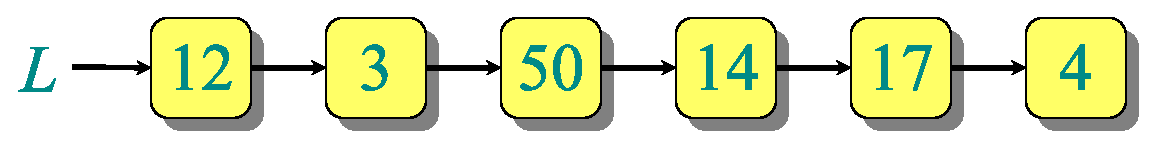
\includegraphics[width=3in]{lecture14/list.eps}
  \caption{Список L}
  \label{fig:list}
\end{figure}

Пример:
\begin{itemize}
\item доступ к элементу с ключом 14 (четвёртый элемент) стоит 4
\item обмен элементов с ключами 3 и 50 стоит 1
\end{itemize}

Поскольку стоимость доступа зависит от позиции элемента, то для уменьшения общих
расходов следует передвинуть те элементы, доступ к которым требуется наиболее
часто, в начало списка.

\section{Онлайн и оффлайн алгоритмы}

\textbf{Определение}: последовательность операций $S$ предоставляется по одной
операции за раз. Для каждой из операций \emph{онлайн-алгоритм} $A$ должен
выполнять эту операцию незамедлительно, безо всякого знания о последующих
операциях последовательности. Пример: игра тетрис.

\emph{Оффлайн-алгоритм} может использовать знание сразу о всей
последовательности операций (``видит'' всю последовательность $S$ наперёд).

Наша цель -- минимизировать полную стоимость всех операций алгоритма $C_A(S)$

\section{Анализ}

Проведём анализ наихудшего случая:

В худшем случае у нас есть противник, который знает как расположены элементы в
списке и с целью максимизации времени будет намеренно запрашивать каждый раз тот
элемент, который расположен в списке последним. Таким образом, оценка полной
стоимости такова:
$$
C_A(S) = \Omega(|S| \cdot n)
$$

Теперь проведём анализ среднего случая.

Предположим что к элементу $x$ доступаются с вероятностью $p(x)$, тогда
ожидаемая общая стоимость будет равна:

$$
E(C_A(S)) = \sum_{x \in L} p(x) \cdot rank_L(X)
$$

это минимизируется, если элементы отсортированы в порядке уменьшение
вероятности.

Эвристики:
\begin{itemize}
\item поддерживать массив, в котором будет хранится количество доступов для
  каждого элемента и поддерживать этот массив в отсортированном состоянии вместе
  с исходным списком элементов
  
\item перемещение в начало (\emph{move to front}, \emph{MTF}) -- после доступа к
  элементу передвинуть его в самое начало списка. Это удвоит стоимость доступа,
  т.к. после доступа нужно будет совершить $rank_L(X)$ перестановок:
  
  $$
  cost = 2 \cdot rank_L(X)
  $$

  Эта стратегия обладает так называемым \emph{свойством локальности}, то есть
  хорошо проявляет себя для последовательностей, конкретные элементы которых
  запрашиваются несколько раз подряд или же просто рядом по времени. Как
  показывает опыт, такие последовательности весьма часто встречаются на
  практике.

\end{itemize}

\end{document}

